\documentclass[pdftex,12pt,a4paper]{article}

\usepackage{amssymb}
\usepackage[pdftex]{graphicx}
\usepackage{etoolbox}
\usepackage{paralist}
\usepackage{mathtools}
\usepackage{hyperref}
\usepackage{floatflt}
\usepackage[xindy,nonumberlist]{glossaries}
\usepackage[utf8]{inputenc}
\usepackage[ngerman]{babel}
\usepackage{bookmark}
\usepackage{fancyhdr}
\usepackage{lastpage}
\usepackage[style=authoryear-ibid,backend=biber]{biblatex}
\addbibresource{./bibliography.bib}
\usepackage[ngerman]{babel}
\usepackage[babel,german=quotes]{csquotes}
\usepackage[font=footnotesize,labelfont=bf,justification=raggedright]{caption}
\usepackage{bm}

% Set TOC title
\renewcommand{\contentsname}{Inhalt}
\addto\captionsngerman{\renewcommand{\contentsname}{Inhalt}}

% Set heading
\defbibheading{head}{\section{Quellenverzeichnis}}

\pagestyle{fancy}
\fancyhf{}  % empty header and footer
\fancyhead[L]{\rotatebox{0}{\scalebox{0.5}[0.5]{
\includegraphics{images/BFH_Logo_C_de_100_RGB.png}}}}
\fancyhead[C]{}
\fancyhead[R]{}
\renewcommand{\headrulewidth}{0.4pt}
\fancyfoot[L]{Spieltheorie}
\fancyfoot[C]{}
\fancyfoot[R]{\thepage{} /~\pageref{LastPage}}
\renewcommand{\footrulewidth}{0.4pt}

\newcommand{\HRule}{\rule{\linewidth}{0.5mm}}

\newglossaryentry{tesselation}{name=Tesselation,
    description={zu Deutsch Parkettierung. Frei übersetzt nach \citeauthor{schwartzman1994words}. `Von dem lateinischen Wort \textit{tessera} ``eine viereckige Tafel'' oder ``ein Würfel, benutzt zum Spielen''. Das lat. Wort \textit{tessera} wurde sehr wahrscheinlich von dem griechischen Wort tessares, was soviel wie ``vier'' bedeutet, abgeleitet bzw.\ ausgeliehen, da ein quadratisches Feld über vier Seiten verfügt. Die Kurzform von tessera war \textbf{tessella}, ein kleines, quadratisches Stück Stein oder eine kubische Kachel, wie sie bei Mosaik zur Verwendung kommt. Da ein Mosaik sich über eine gegebene Fläche ersttreckt, ohne eine Region auszulassen, ist die geometrische Bedeutung des Wortes tessellieren ``eine Ebene mit einem Muster bedecken, so dass keine Region unbedeckt bleibt.''. Raum oder Hyperraum kann auch tesseliert werden (\citeyear{schwartzman1994words})}
}

\newglossaryentry{dualGraph}{name=Dualer Graph,
    description={Gegeben sei $G$, ein kreuzungsfreier, nicht leerer und zusammenhängender Graph. Wie~\cite{klein2005algorithmischegeometrie} angibt, ist ein Graph $G*$ dann dual zu $G$, wenn Folgendes gilt:
    \begin{compactitem}
    \item Im Innern jeder Fläche von $G$ werden neue Punkte $p_F^*$ hinzugefügt. Dies sind die Knoten von $G^*$.
    \item Für jede Kante $e$ (edge) von $G$, welche die angrenzenden Flächen $F$ und $F'$ besitzt, werden die Punkte $p_F^*$ und $p_{F'}^*$ zu einer Kante $e^*$ verbunden. Diese kreuzt nur die Kante $e$ und sonst keine andere Kante.
    \end{compactitem}
    Wenn dies gilt, dann ist $\boldsymbol{G^*}$ der \textbf{\textit{duale Graph}} von $G$. ${(G^*)}^*$ ist wiederum zum Graphen $G$ äquivalent}
}


\newglossaryentry{bigOh}{name=Gross-Oh $O()$,
    description={Die Gross-Oh-Notation $O$ besagt, dass eine Funktion maximal das asymptotische Wachstumsverhalten der angegebenen Funktion aufweist, beispielsweise:
\noindent\hspace*{10mm}%
$g \in O(f)$
Dies besagt, dass die Funktion $g$ in ihrem asymptotischen Wachstum praktisch überall (bis auf einen konstanten Faktor) durch die Funktion $f$ beschränkt ist.
Sie bildet also eine Art obere Schranke. Frei nach~\citeauthor{goodrich2002algorithm} übersetzt (\citeyear[S. 13]{goodrich2002algorithm})}
}

\newglossaryentry{bigOmega}{name=Gross-Omega $\Omega()$,
    description={Die Gross-Omega-Notation $\Omega$ definiert eine untere Schranke, welche besagt, dass eine Funktion bis auf einen konstanten Faktor in ihrem asymptotischen Wachstum grösser oder gleich einer anderen Funktion ist,
beispielsweise:
\noindent\hspace*{10mm}%
$g \in \Omega(f)$
Wodurch auch $f \in O(g)$ gilt. Frei nach~\citeauthor{goodrich2002algorithm} übersetzt (\citeyear[S. 16 bis 17]{goodrich2002algorithm})}
}

\newglossaryentry{bigTheta}{name=Gross-Theta $\Theta()$,
    description={Die Gross-Theta-Notation $\Theta$ erlaubt es, zu sagen, dass zwei Funktionen $g$ und $f$ bis zu einem konstanten Faktor dasselbe asymptotische Wachstumsverhalten aufweisen, beispielsweise:
\noindent\hspace*{10mm}%
$g \in \Theta(f)$
Wodurch auch $g \in O(f)$ und $g \in \Omega(f)$ gilt. Frei nach~\citeauthor{goodrich2002algorithm} übersetzt (\citeyear[S. 16 bis 17]{goodrich2002algorithm})}
}

\newglossaryentry{simplex}{name=Simplex,
  description={Eine konvexe Hülle von $n + 1$ Punkten im $\mathbb{R}^d$, $n <= d$, die nicht in einem $(n - 1)$-dimensionalen Teilaraum liegen, nennt man das Simplex der Dimension $n$~\parencite[S. 23]{klein2005algorithmischegeometrie}}
}

\newglossaryentry{bisector}{name=Bisektor,
  description={Eine Gerade zwischen zwei Punkten, bestehend aus Punkten, welche genau denselben Abstand zu den zwei Punkten haben~\parencite[S. 25]{klein2005algorithmischegeometrie}}
}

\newglossaryentry{euclideanDistance}{name=Euklidischer Abstand,
  description={Bestimmt den Abstand zweier Punkte. $|x_i - x_j| = \sqrt{{\sum_{k=1}^{m} {(x_ik - x_jk)}^2}}$~\parencite[S. 16]{atsuyuki2000spatialtessellations}}
}

\newglossaryentry{convexHull}{name=Konvexe Hülle,
  description={Informell gesagt handelt es sich dabei um die Hülle eines Gummibandes, welches um eine Punktemenge in der Ebene gelegt wird. Oder, etwas formeller: ``Eine Region $R$ ist \textbf{konvex}, wenn jederzeit gilt, dass sich zwei Punkte $p$ und $q$, sowie deren Liniensegment $\overline{pq}$ in $R$ befinden. Die \textbf{konvexe Hülle} einer Punktemenge $S$ ist der Umfang der schmalsten konvexen Region, welche alle Punkte von $S$ beinhaltet bzw\. auf deren Rand hat.''. Frei nach~\citeauthor{goodrich2002algorithm} übersetzt (\citeyear[S. 572 bis 576]{goodrich2002algorithm})}
}

\makeglossaries{}
% Add all glossary entries no matter if they get
% referenced or not
\glsaddall{}

\setlength{\headheight}{32pt}
\setlength{\abovecaptionskip}{2pt plus 3pt minus 2pt}
\setlength{\parindent}{0pt}
\setlength{\parskip}{10pt plus 1pt minus 1pt}

\apptocmd{\sloppy}{\hbadness10000\relax}{}{}

% Add all bibliography entries no matter if they
% get cited or nod
\nocite{*}

\begin{document}
%deckblatt start
\thispagestyle{empty}
\begin{center}
\rotatebox{0}{\scalebox{1.0}[1.0]{
\includegraphics{images/BFH_Logo_C_de_100_RGB.png}}}\\
\end{center}
\begin{center}
\Large{Berner Fachhochschule (BFH)}\\
\end{center}
 
 
\begin{center}
\Large{Departement Informatik}
\end{center}
\begin{verbatim}
\end{verbatim}
\begin{center}
\textbf{\LARGE{BTI7501p --- Spieltheorie}}
\end{center}
\begin{verbatim}
 
 
\end{verbatim}
\begin{center}
\textbf{Bericht}
\end{center}
\begin{verbatim} 
\end{verbatim}
 
\begin{flushleft}
\begin{tabular}{lll}
\textbf{Thema:} & & Projektarbeit `Damespiel'\\
& & \\
& & \\
    \textbf{Studenten:} & & Thi Thuy-Duc Dao (daodt1@bfh.ch), Sven Osterwalder (ostes2@bfh.ch)\\
\textbf{Date:} & & {\today}\\
\textbf{Professor:} & & Prof.\  Dr.\ Jürgen Eckerle
\end{tabular}
\end{flushleft}

\newpage
\tableofcontents
\newpage
\section{Einleitung}
\label{sec:introduction}
Die vorliegende Arbeit wurde im Rahmen der Projektarbeit des Moduls BTI7501p --- Spieltheorie verfasst.

Der erste Teil stellt die Aufgabenstellung und Projektvorgaben vor. Im zweiten Teil wird die eigentliche Implementation der Aufgabe vorgestellt.

Diese schriftliche Arbeit dient als Ergänzung zum Vortrag in diesem Modul.
Der Text kann jedoch auch eigenständig betrachtet werden.

\section{Aufgabenstellung}
\label{chap:basics}
Bei der Projektaufgabe `Damespiel' geht es grundsätzlich darum eine Art künstliche Intelligenz --- basierend auf den vorgstellten Algorithmen des Moduls --- zu entwickeln, welche fähig ist eine Urform des Damespiels autonom und möglichst optimal zu spielen.

\subsection{Spielbrett}
\label{sec:board}
Als Spielbrett dient dabei eine modifizierte Version des klassichen Schachbretts --- ein Spielbrett mit abwechselnd schwarzen und weissen Feldern der Grösse 5 auf 5. Es existeren zwei Parteien, eine Partei mit schwarzen und eine Partei mit weissen Steinen.Jede Partei erhält dabei 12 Steine. Im Gegensatz zum klassischen Damespiel, wo nur die schwarzen Felder mit Steinen besetzt werden, werden alle Felder mit Steinen besetzt. Die Verteilung ist so, dass die Steine der Spieler auf je eine Hälfte aufgeteilt werden. Die mittlere Reihe enthält dann jeweils zwei Steine pro Partei, das mittlere Feld bleibt leer.

\begin{figure}[h]
\centering

\includegraphics[width=200px]{images/checkers_board.png}
\caption[width=100px]{Darstellung Spielbrett mit Initialstellung\protect\footnotemark}
\label{fig:checkersBoardInitial}
\end{figure}
\footnotetext{Eigene Darstellung mittels Libre Office Impress und Gimp}

\subsection{Regeln}
\label{sec:rules}
Im Spiel wird abwecheslungsweise gespielt und pro Zug darf maximal ein Stein gezogen werden. Grundsätzlich sind alle Bewegungsrichtungen möglich --- sofern das angestrebte Feld frei ist. Ist ein Feld von einem gegenrischen Stein blockiert, das direkt hinter dem Stein liegende Feld aber frei, so darf der gegnerische übersprungen werden. Dabei wird der übersprungene Stein vom Feld entfernt. Im Gegensatz zur klassischen Variante des Damespiels gibt es in der hier beschriebenen Variante keine Ketten. Dies heisst, dass ein Spieler mit einem Stein gleich mehrere gegnerische Steine nacheinander überpspringen kann. Dabei gilt die zuvor beschriebene Regel.

\begin{minipage}[t]{0.4\textwidth}
    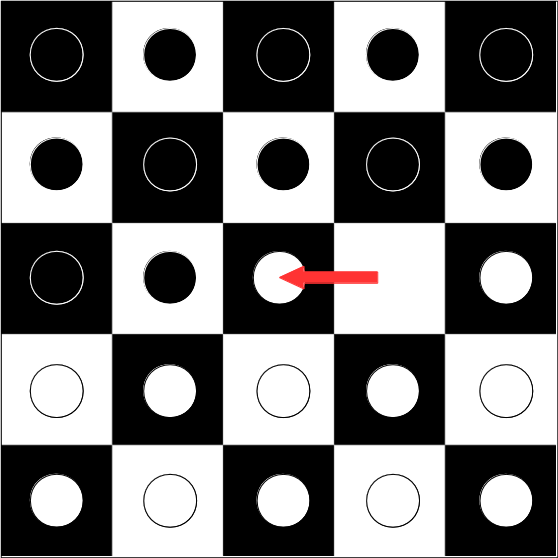
\includegraphics[width=\textwidth]{images/checkers_rule_01.png}
    \captionof{figure}{Seitwärtsbewegung eines weissen Steins\protect\footnotemark}
\label{fig:checkersRule01}
\end{minipage}
\footnotetext{Eigene Darstellung mittels Libre Office Impress und Gimp}
\begin{minipage}[t]{0.4\textwidth}
    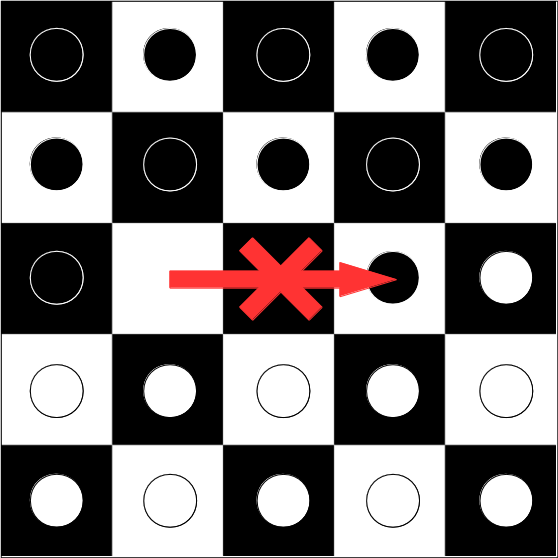
\includegraphics[width=\textwidth]{images/checkers_rule_02.png}
    \captionof{figure}{Ein schwarzer Stein übersrpingt einen weissen Stein\protect\footnotemark}
\label{fig:checkersRule02}
\end{minipage}
\footnotetext{Eigene Darstellung mittels Libre Office Impress und Gimp}

\newpage
\section{Umsetzung}
\label{sec:implementation}

Die Umsetzung des Projektes basiert auf einem objektorientierten Ansatz und nutzt Python 2.7.7.

\subsection{Module}
\label{subsec:modules}
Zur Umsetzung der Applikation wurde diese, wie in Abbildung~\ref{fig:module_structure} ersichtlich, in die folgenden Module unterteilt:

\begin{compactitem}
\item \textit{algorithms}\\
    Enthält Algorithmen zur Lösungsfindung
\item \textit{controller}\\
    Enthält die komplette Steuerung des Spiels, sowie die grundlegenden Elemente
\item \textit{player}\\
    Enthält Spieler zur Durchführung des Spiels
\end{compactitem}

\begin{minipage}[]{1.0\textwidth}

    \centering
    \begin{minipage}[t]{0.5\textwidth}
        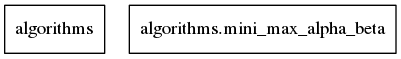
\includegraphics[width=\textwidth]{images/packages_algorithms.png}
    \end{minipage}
    \begin{minipage}[t]{0.3\textwidth}
        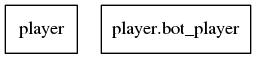
\includegraphics[width=\textwidth]{images/packages_player.png}
    \end{minipage}
    \begin{minipage}[t]{0.95\textwidth}
        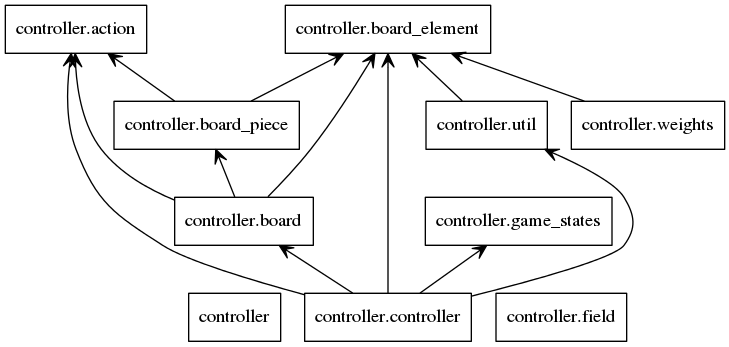
\includegraphics[width=\textwidth]{images/packages_controller.png}
    \end{minipage}

\captionof{figure}{Modulstruktur der Applikation\protect\footnotemark}
\label{fig:module_structure}
\end{minipage}
\footnotetext{Eigene Darstellung mittels Pyreverse (http://www.logilab.org/blogentry/6883)}

\newpage

\subsection{Klassenstruktur}
\label{subsec:class_structure}
Die Applikation besteht aus den in der Abbildung~\ref{fig:class_structure} abgebildeten Klassen und Attributen.

\begin{minipage}[]{1.0\textwidth}

    \centering
    \begin{minipage}[t]{0.2\textwidth}
        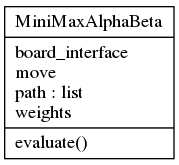
\includegraphics[width=\textwidth]{images/classes_algorithms.png}
    \end{minipage}
    \begin{minipage}[t]{0.22\textwidth}
        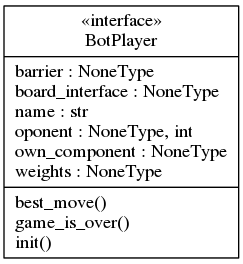
\includegraphics[width=\textwidth]{images/classes_player.png}
    \end{minipage}
    \begin{minipage}[t]{0.7\textwidth}
        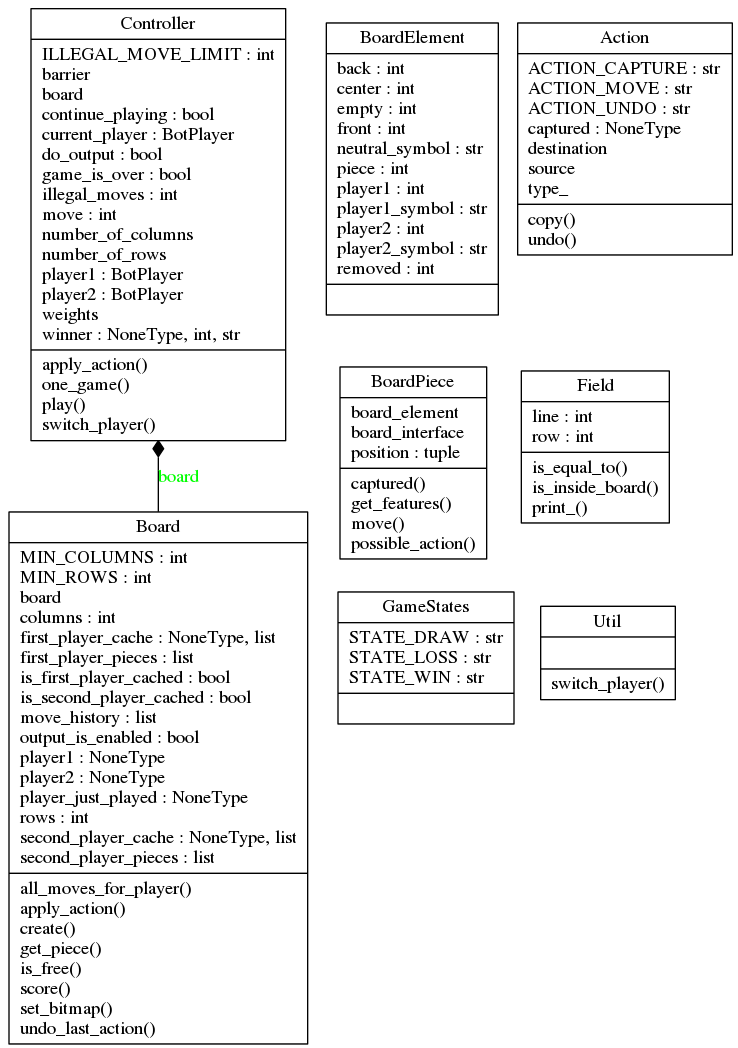
\includegraphics[width=\textwidth]{images/classes_controller.png}
    \end{minipage}

\captionof{figure}{Klassendiagramm der Applikation\protect\footnotemark}
\label{fig:class_structure}
\end{minipage}
\footnotetext{Eigene Darstellung mittels Pyreverse (http://www.logilab.org/blogentry/6883)}

\subsection{Programmablauf}
\label{subsec:program_flow}

Grundsätzlich ist die Applikation so aufgebaut, dass sie direkt mittels dem Controller-Interface initialisiert und dann gestartet werden kann. Die Berechnung bzw.\ der Ablauf des Spiels läuft dann vollkommen automatisch ab. Schlussendlich wird eine Meldung über den Gewinner bzw.\ ob ein Unentschieden erreicht wurde ausgegeben.

Der hauptsächliche Teil des Programmablaufs findet --- wie der Name bereits andeutet --- im \textit{Controller}-Modul statt. Dieses startet eine Schleife, welche so lange läuft, wie das Spiel nicht beendet ist. Zusätzlich wurde eine Limit eingebaut, welche nach Erreichen das Spiel mit einem Unentschieden abbricht. Dies wurde so gewählt, da es möglich ist, dass keine Relevanten Züge mehr geschehen und es so unter Umständen --- bei einer sehr passiven Strategie der Spieler --- zu keinem Ende kommt.

Innerhalb der Schleife wird quasi Zug nach Zug pro Spieler berechnet, wobei pro Zug die Seite gewechselt wird. Für jeden Spieler wird pro Zug vom Controller aus der beste Zug abgefragt. Der Spieler evaluiert dies, indem er alle möglichen Züge durch das Interface des Spielbretts abfragt und dann mittels einem gewählten Algorithmus eine Evaluation --- bis zu einer gewissen Tiefe --- durchführt. Die Schnittstelle des Spielers ist generisch gehalten, so dass ein Spieler im Prinzip einen beliebigen Algorithmus zur Evaluation des besten Zuges anwenden kann. Aktuell wurde jedoch nur der MiniMax-Algorithmus mit Alpha-Beta-Pruning umgesetzt.

Hat der Spieler einen von ihm aus gesehen besten Zug evaluiert, meldet er dies dem Controller, welcher dann den Zug durch das Interface des Spielbretts auf dieses anwendet. Als Abbruchkriterium dient hier ob ein Spieler entweder keine Steine mehr zur Verfügung hat oder aber ein Spieler keine erlaubten Züge (Bewegung auf ein freies Feld, Überspringung des Gegners) vornehmen kann.

In den Abbildungen~\ref{fig:program_flow_01} und~\ref{fig:program_flow_02} wird das gerade Genannte visuell verdeutlicht.

\newpage

\begin{minipage}[]{1.0\textwidth}

    \centering
    \begin{minipage}[t]{0.7\textwidth}
        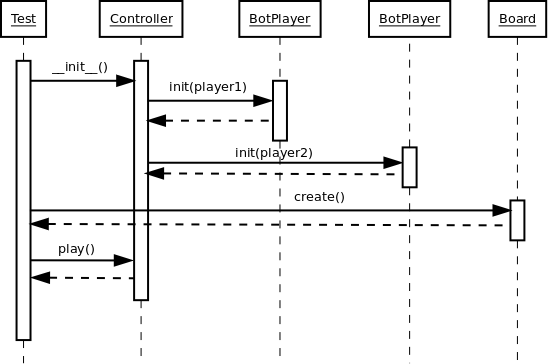
\includegraphics[width=\textwidth]{images/program_flow_01.png}
        \captionof{figure}{Initialisation der Applikation\protect\footnotemark}
\label{fig:program_flow_01}
    \end{minipage}

    \hspace{1cm}

    \begin{minipage}[t]{0.8\textwidth}
\label{fig:program_flow_02}
        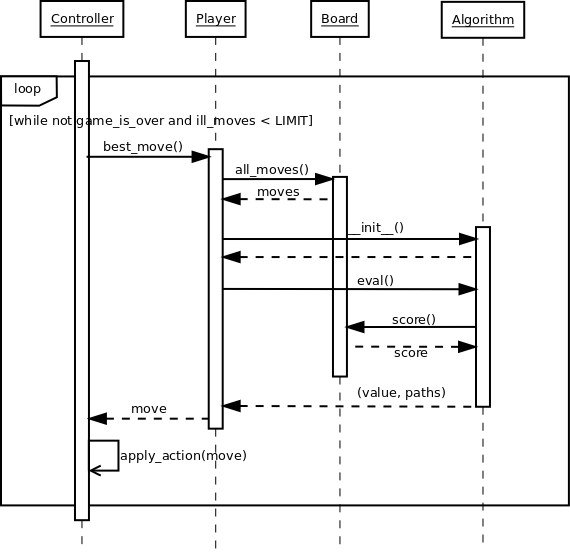
\includegraphics[width=\textwidth]{images/program_flow_02.png}
        \captionof{figure}{Eigentlicher Ablauf der Applikation\protect\footnotemark}
\label{fig:program_flow_02}
    \end{minipage}
\end{minipage}
\addtocounter{footnote}{-2} %3=n
 \stepcounter{footnote}\footnotetext{Eigene Darstellung mittels Dia}
 \stepcounter{footnote}\footnotetext{Eigene Darstellung mittels Dia}


\newpage
\section{Fazit und Ausblick}
\label{chap:ending}

Die Projektarbeit im Rahmen des Modules \textit{"BTI7501p --- Spieltheorie"} war sehr spannend und hat bei der Umsetzung viel Spass gemacht. Mit dem Ziel die Urform des Damespiels umzusetzen wurde unserer Meinung nach ein guter Mittelweg betreffend der Komplexität der Aufgabenstellung gewählt --- das Projekt wurde nicht zu aufwändig, man konnte dennoch das Gelernte praktisch Umsetzen.

Da die Applikation Modular aufgebaut ist, ist es ohne Weiteres möglich weitere Spieler zu implementieren, welche z.B. andere Bewertungsfunktionen nutzen und so etwas Variation in das Spiel zu bringen. Auf der algorithmischen Ebene liesse sich sicherlich viel mehr umsetzen, so wäre beispielsweise eine Implementation des \textit{Negmax}-Algorithmus spannend, oder aber der Einsatz von \textit{Backtracking} oder beispielsweise der \textit{Aspiration Search} Algorithmus, um nur Einige zu nennen.

\newpage
\printbibliography[heading=head]
\newpage
\printglossary[numberedsection]
\end{document}
